\documentclass{perassignments}



\usepackage{hyperref}
\usepackage[abjad]{pertheorems}
\usepackage{mathtools}
\usepackage{amsmath}
\usepackage{float}
\usepackage{common}
\usepackage{xepersian}




\settextfont[]{XBNiloofar}
%\setmathdigitfont{XBTabriz}


\CourseName[آز شبکه‌]
\Semester[اول]
\Year[01]
\Prof[دکتر صفائی]
\Dept[دانشکده مهندسی کامپیوتر]
\CollabFirst[عماد زین‌اوقلی]{98103267}
\CollabSecond[پارسا رییسی]{98103223}
\CollabThird[سیدابوالفضل رحیمی ]{97105941}

\renewcommand{\maketitle}{\MakeMyLabTitle}
\allowdisplaybreaks


\begin{document}
	\maketitle
	\section{آزمایش}
	سناریو زیر را به صورت خواسته شده طراحی کردیم.
	\begin{figure}[H]
		\centering
		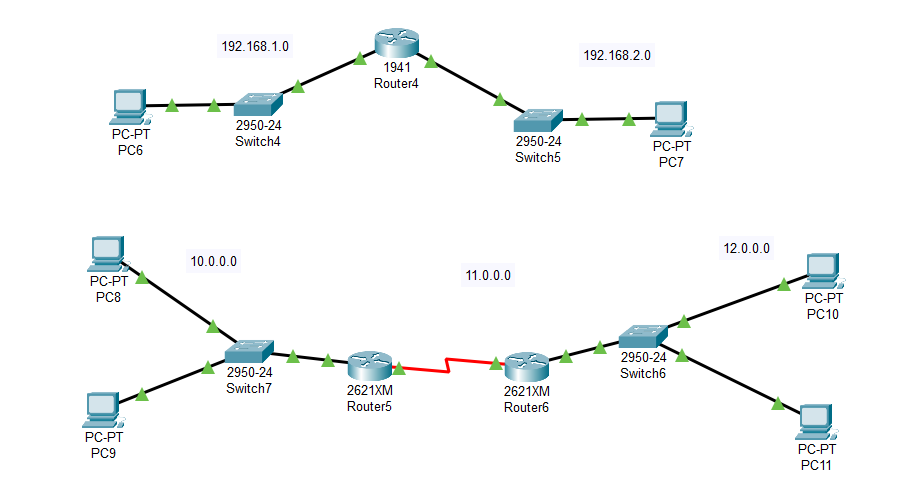
\includegraphics[width= 0.7\linewidth]{graphics/a.png}
		\caption{طرح سناریو}
		\label{fig:a}
	\end{figure}
	\subsection{سوال ۱}
	دستور 
	\texttt{?}
	را وارد کردیم و جواب‌های
	\ref{fig:b}, \ref{fig:c} 
	 زیر برگردانده شد. 
		\begin{figure}[H]
		\centering
		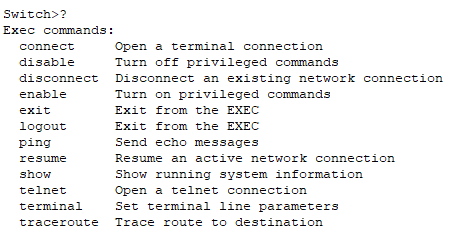
\includegraphics[width= 0.7\linewidth]{graphics/b.png}
		\caption{دستورات سوییج}
		\label{fig:b}
	\end{figure}
		\begin{figure}[H]
	\centering
	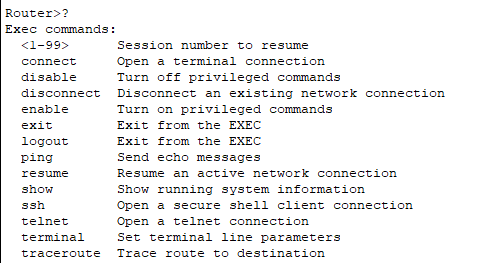
\includegraphics[width= 0.7\linewidth]{graphics/c.png}
	\caption{دستورات روتر}
	\label{fig:c}
\end{figure}
	\subsection{سوال ۲}
	دستور 
	\lr{\texttt{show running-config}}
	تنظیمات سوییچ 
	\ref{fig:d}
	و یا روتر
	\ref{fig:e}
	 نشان می‌دهد.
	 \begin{figure}[H]
	 	\centering
	 	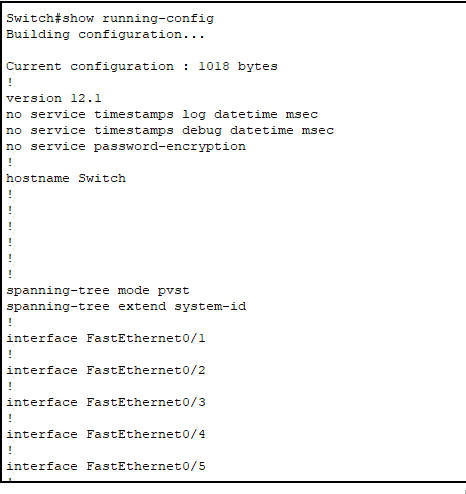
\includegraphics[width= 0.7\linewidth]{graphics/d.png}
	 	\caption{دستور 	\lr{\texttt{show running-config}} سوییج}
	 	\label{fig:d}
	 \end{figure}
	 \begin{figure}[H]
	 	\centering
	 	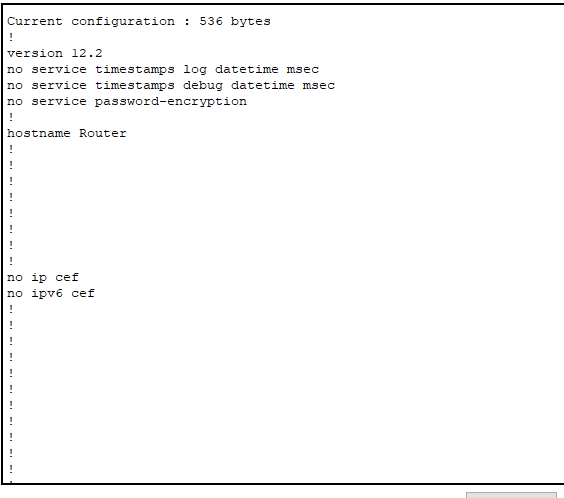
\includegraphics[width= 0.7\linewidth]{graphics/e.png}
	 	\caption{دستور 	\lr{\texttt{show running-config}} روتر}
	 	\label{fig:e}
	 \end{figure}
	 دستور 
	 \lr{\texttt{show ip route}}
	 بر روی روتر 
	 \ref{fig:f}, \ref{fig:f1}
	مسیر‌های مشخص شده در روتر نشان می‌دهد. 
	 \begin{figure}[H]
	 	\centering
	 	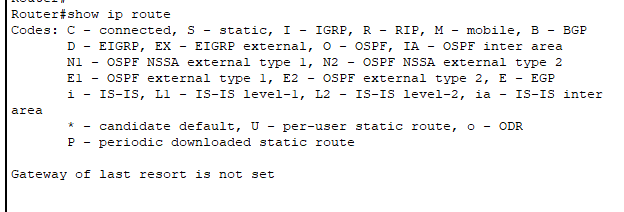
\includegraphics[width= 0.7\linewidth]{graphics/f.png}
	 	\caption{
	 		دستور	
	 		 	\lr{\texttt{show ip route}} 
	 		 	در روتر قبل از تنظیمات.}
	 	\label{fig:f}
	 \end{figure}
	 \begin{figure}[H]
	 	\centering
	 	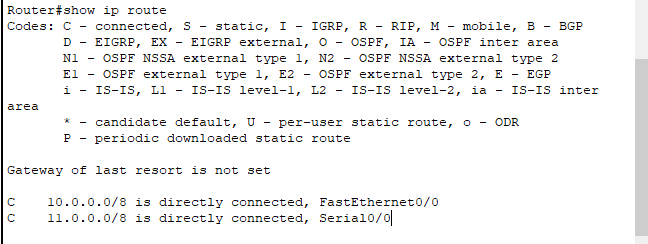
\includegraphics[width= 0.7\linewidth]{graphics/f1.png}
	 	\caption{
	 		دستور	
	 		\lr{\texttt{show ip route}} 
	 		در روتر بعد از تنظیمات.}
	 	\label{fig:f1}
	 \end{figure}
 	دستور 
 	\lr{\texttt{show mac address-table}}
 	بر روی سوییج 
 	\ref{fig:g},\ref{fig:g1}
 	سوییچ‌های قعلا را نشان می‌دهد. 
 	\begin{figure}[H]
 		\centering
 		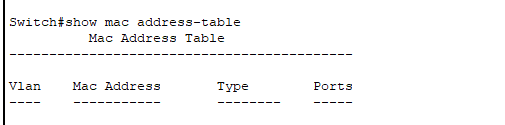
\includegraphics[width= 0.7\linewidth]{graphics/g.png}
 		\caption{
 			دستور	
 			\lr{\texttt{show mac address-table}} 
 			در سوییچ قبل از تنظیمات.}
 		\label{fig:g}
 	\end{figure}
 	\begin{figure}[H]
 		\centering
 		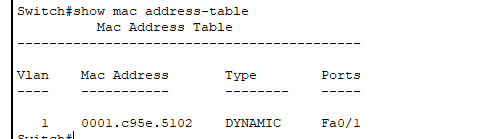
\includegraphics[width= 0.7\linewidth]{graphics/g1.png}
 		\caption{
 			دستور	
 			\lr{\texttt{show mac address-table}} 
 			در سوییچ بعد از تنظیمات.}
 		\label{fig:g1}
 	\end{figure}
 	دستور 
 	\lr{\texttt{show interface brief}}
 	در سوییچ  
 	\ref{fig:i}
 	interfaceها
 	و وضعیت آن‌ها را و در روتر
 	\ref{fig:h}
 	IP 
 	تعیین شده برای آن interface‌ را نشان می‌دهد.
 	\begin{figure}[H]
 		\centering
 		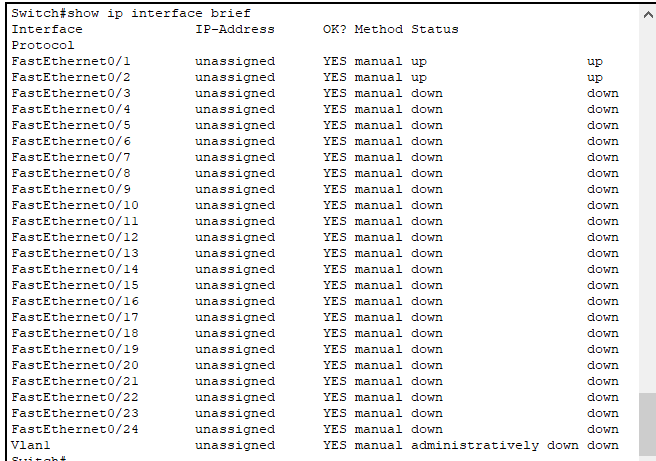
\includegraphics[width= 0.7\linewidth]{graphics/i.png}
 		\caption{دستور 	\lr{\texttt{show interface brief}} سوییج}
 		\label{fig:i}
 	\end{figure}
 	\begin{figure}[H]
 		\centering
 		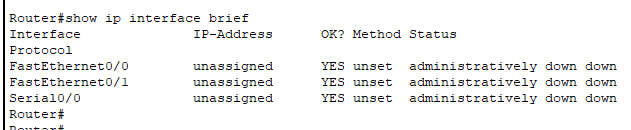
\includegraphics[width= 0.7\linewidth]{graphics/h.png}
 		\caption{دستور 	\lr{\texttt{show interface brief}} روتر}
 		\label{fig:h}
 	\end{figure}
 	دستور 
 	\lr{\texttt{show vlan brief}}
 	بر روی سوییج 
 	\ref{fig:k}
 	اطلاعات مربوط به پورت‌های vlan را نشان می‌دهد. 
 	\begin{figure}[H]
 		\centering
 		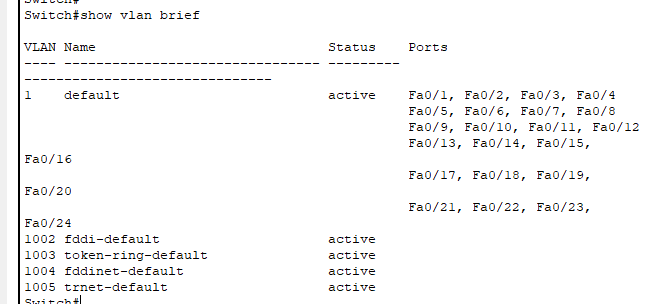
\includegraphics[width= 0.7\linewidth]{graphics/k.png}
 		\caption{
 			دستور	
 			\lr{\texttt{show vlan brief}} 
 			در سوییچ.}
 		\label{fig:k}
 	\end{figure}
 	\subsection{سوال ۳}
 	Gateway
 	رابط بین دو شبکه متفاوت با پروتکل‌های متفاوت است. Gateway‌ها همانند دروازه‌ای هستند که داده برای ورود و یا خروج از شبکه -- این شامل ترافیک داخلی نمی‌شود-- لازم است که از آن بگذرند.
 	\subsection{ping}
 	پس از وارد کردن تنظیمات مربوط، دستور 
 	\lr{\texttt{ping 192.168.2.2}}
 	را بر روی کامپیوتر با آدرس 
 	\lr{\texttt{192.168.1.2}}
 	اجرا کردیم
 	\ref{fig:n}.
 	 	\begin{figure}[H]
 		\centering
 		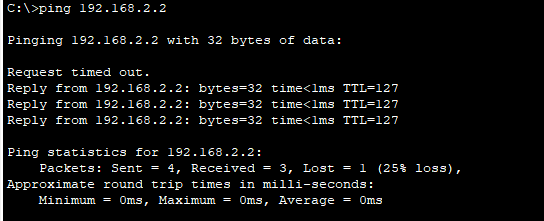
\includegraphics[width= 0.7\linewidth]{graphics/n.png}
 		\caption{
 			دستور	
 			\lr{\texttt{ping}} }
 		\label{fig:n}
 	\end{figure}
\end{document}